\documentclass[10pt,a4paper]{article}
\usepackage{amsmath, amsfonts, amssymb}
\usepackage[utf8]{inputenc}
\usepackage[OT1]{fontenc}
\usepackage{gensymb}
\usepackage[margin=2.5cm, landscape]{geometry}
\usepackage{graphicx}
\usepackage[dvipsnames]{xcolor}
\usepackage{paracol}
\usepackage{calc}
\usepackage{enumitem}
\usepackage[hang, font ={small, it}, labelformat=empty]{caption}
\renewcommand{\figurename}{Fig}

\usepackage[object=vectorian]{pgfornament}

\usepackage{tikz}
\usepackage[uprightgreeks,frenchstyle,light,fulloldstylenums,veryoldstyle]{kpfonts}

\globalcounter{enumi}
\newcommand{\switchenum}{\setcounter{enumi}{\arabic{enumi}-1}\switchcolumn}
\renewcommand{\theenumi}{\S.\arabic{enumi}}

\setlength{\parskip}{1ex}
\setlength{\parindent}{0pt}

\DeclareMathOperator{\tang}{tang.}
\DeclareMathOperator{\cotg}{cot.}
\DeclareMathOperator{\sing}{sin.}
\DeclareMathOperator{\cosg}{cos.}

\pagestyle{empty}

\def\D{\mathrm{d}}

\renewcommand{\rmdefault}{cmr}

\begin{document}
	
	\begin{paracol}{2}
	\par \textit{Nova Acta Eruditorum 1745, p. 523}
	\par E79 (Eneström Index) 
	\begin{center}
		\par \pgfornament[width = 0.8\linewidth]{88}
		
		\par {\bf Problema geometricum, propositum}\\
		publice ab anonymo geometra
	\end{center}
	\switchcolumn
	\par \textit{Nova Acta Eruditorum 1745, p. 523}
	\par E79 (Eneström Index) 
	\begin{center}
		\par \pgfornament[width = 0.8\linewidth]{88}
		
		\par {\bf Voorstel tot een meetkundig probleem}\\
		publiek door een anomnieme meetkundige
	\end{center}
	\switchcolumn*
	
	
	\par Proposito puncto $F$ invenire omnes curves $AMBN$ huius naturae, ut singuli radii ex $F$ egressi post duplicem reflectionem in $M$ \& $N$ in idem punctum $F$ revertantur.  Primum quidem perspicuum est omnes ellipses, quae in $F$ habeant alterutrum focum, quaesito satisfacere.  Sed praeterea dantur innumerabiles aliae curvae, eadem indole gaudentes, quarum investigatio limites analyseos non parum extendere videtur.
		
	\switchcolumn
	\par Gegeven een punt $F$, vind alle krommen $AMBN$ zodat, elke straal vanuit $F$, na twee terugkaatsingen in $M$ \& $N$, terug in het originele punt $F$ terechtkomt. Een eerste van zo'n soort krommen zijn alle ellipsen, die een brandpunt hebben in het punt $F$. Maar er kunnen ontelbaar veel andere krommen gegeven worden die dezelfde eigenschap hebben, de wijze om deze analytisch te onderzoeken is nog niet gezien.

	\switchcolumn*
			
	\begin{figure}[h]
		\centering
		\par {
			\fontfamily{jkplvos}\selectfont
			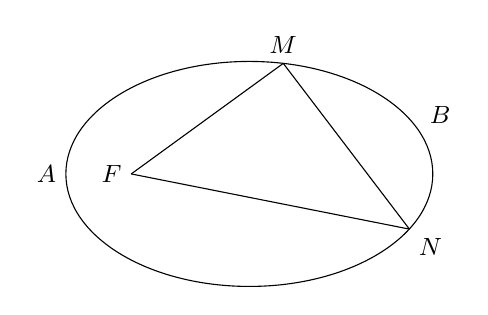
\begin{tikzpicture}[yscale=0.8]
			\draw [rotate around={0:(1.5,0)}] (1.5,0.) ellipse (2.33cm and 1.786cm);
			\draw (0,0)-- (1.931,1.755);
			\draw (1.931,1.755)-- (3.533,-0.876);
			\draw (3.5330,-0.876)-- (0,0);
			\draw (0,0) node [left] {\small $F$};
			\draw (1.93,1.75) node [above] {\small $M$};
			\draw (3.53,-0.87) node [below right] {\small $N$};
			\draw (-0.83,0) node [left] {\small $A$};
			\draw (3.67,0.64) node [above right] {\small $B$};
			\end{tikzpicture}}
		\fontfamily{cmr}\selectfont
		\caption{Tab. III. Fig. 3.}
	\end{figure}
	\switchcolumn
	\begin{figure}[h]
		\centering
		\par {
			\fontfamily{jkplvos}\selectfont
			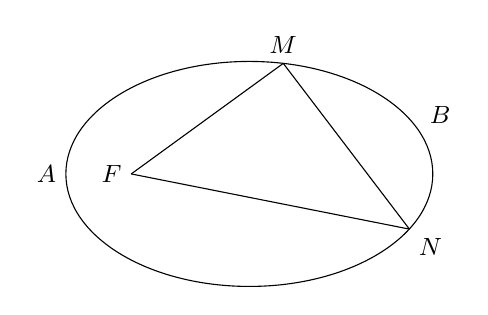
\begin{tikzpicture}[yscale=0.8]
			\draw [rotate around={0:(1.5,0)}] (1.5,0.) ellipse (2.33cm and 1.786cm);
			\draw (0,0)-- (1.931,1.755);
			\draw (1.931,1.755)-- (3.533,-0.876);
			\draw (3.5330,-0.876)-- (0,0);
			\draw (0,0) node [left] {\small $F$};
			\draw (1.93,1.75) node [above] {\small $M$};
			\draw (3.53,-0.87) node [below right] {\small $N$};
			\draw (-0.83,0) node [left] {\small $A$};
			\draw (3.67,0.64) node [above right] {\small $B$};
			\end{tikzpicture}}
		\fontfamily{cmr}\selectfont
		\caption{Tab. III. Fig. 3.}
	\end{figure}
	\end{paracol}
\end{document}